\setchapterstyle{kao}
\setchapterpreamble[u]{\margintoc}
\chapter{Digital interfaces for environmental sensors}
\labch{digital_interfaces}

In \refch{circuits_intro}, we considered the fundamentals of constructing circuits that exploit the abilities of microcontrollers to measure voltage and time to quantify environmental variables.
These circuits were based on \textit{analog} sensors -- that is, sensors that return signals in the form of continuously variable voltages or time lags.
By integrating the microcontroller, circuit and analog sensor components, you assembled a device that provided a \textit{digital} signal -- a number that represents an observation of the corresponding environmental parameter.

A modern trend in sensor development is \textit{digital sensors}, whose output is intrinsically in the form of numbers rather than voltage or time.
If you used the external \DS3231 Real Time Clock in \refch{time_keeping}, you have already used a digital sensor.
In digital sensors, the circuitry and some of the microcontroller functions that you used to convert analog signals to digital outputs have been placed on the sensor itself.
This means that the user-designed circuitry and microcontroller interfaces can usually be greatly simplified compared to an analog sensor measuring the same quantity.

Because digital sensors typically return observations as numbers with many decimal places, it's tempting to overlook the fact that in many cases they may be less accurate and precise than analog sensors (or may cost more for comparable accuracy and precision).
It's important to keep in mind that digital sensors have the same basic operating principles and limitations as analog sensors.
The internal circuitry of digital sensors is designed by experts and mass-produced in sophisticated factories.
This means that the tradeoffs and optimizations in sensitivity, resolution, power consumption, \etc that you considered in working with analog sensors have been decided by highly skilled professionals.
Remember, though, that these circuits (and hence the digital sensors that use them) still have most of the same constraints you wrestled with in your own sensor design.

With those caveats in mind, digital sensors often have a number of advantages relative to analog sensors.
Depending on the type of digital sensor and the context, these advantages may include:
\begin{itemize}
	\item Digital sensors use digital \texttt{GPIO}s, which are more abundant than analog \texttt{GPIO}s on most microcontrollers;
	\item Protocols for communicating with digital sensors are two-way -- information such as settings, commands to take readings \etc can be sent to digital sensors to make them more efficient and versatile;
	\item Some digital sensor protocols support multiple sensors on one set of \texttt{GPIO}s and wires, with microcontrollers able to identify and query each of those sensors individually;
	\item Some digital protocols support very long wire connections (though others are limited to very short wires);
	\item Some digital sensors internally do complex computations, such as integrating angular orientation from angular accelerations, which would be expensive in terms of processor cycles and energy to perform on a microcontroller.
\end{itemize}
These advantages are evident in many industrial applications (cars, phones, \etc).
As a result, many useful digital environmental sensors are mass produced and amazingly cheap for their capabilities.

This chapter uses examples of readily available and scientifically informative environmental sensors to illustrate how to use several common communication protocols for digital sensors.
Many other examples using each of these protocols appear later in this book, in applications of data from digital sensors to drawing inferences and hypothesis testing about environmental mechanisms.
For some readers, one or two of these protocols may be sufficient for the examples and data collection applications at hand.
If so, it may be an efficient strategy to focus on that subset of protocols, returning to learn the others if and when the need arises.

\subsection{Communicating with digital sensors}
In practice, getting measurements from digital sensors usually involves two main elements: establishing the appropriate circuit connections, and finding (or, occasionally, writing) a \emph{driver}.
A driver is a piece of code that interfaces between a microcontroller and digital sensor.
The driver enables the user to interact with a digital sensor, \eg by setting measurement parameters or querying for data, with simple, intuitive high-level \Micropython commands.
The driver handles messages between the microcontroller and the digital sensor at a very low level, that takes some technical expertise and patience to understand.
Fortunately, \Micropython-based drivers are freely available online for many of the most useful digital environmental sensors, and more are being written all the time.
You typically don't need to know much about the inner workings of a driver to use it for obtaining environmental sensor readings.

Most digital sensors used in environmental sensing communicate using one of four protocols:

%\begin{itemize}
%	\item \textbf{Inter-Integrated Circuit (\i2c)}
%
%	The \htmladdnormallink{\i2c}{https://en.wikipedia.org/wiki/I\%C2\%B2C} protocol (pronounced ``eye squared sea'') is commonly used in digital sensors for time, light, accceleration, \etc, and is also used in many small TFT displays for microcontrollers.
%	%Adafruit provides a useful \htmladdnormallink{overview of \i2c}{https://learn.adafruit.com/adafruit-ft232h-with-spi-and-i2c-libraries/i2c-devices}.
%	\i2c is a ``2 wire'' protocol (in addition to \texttt{Vin} and \texttt{GND}).
%	\i2c is designed to work over relatively short distances ($\le$ a few meters), but \htmladdnormallink{\texttt{differential extenders}}{https://learn.sparkfun.com/tutorials/qwiic-differential-i2c-bus-extender-pca9615-hookup-guide/all} are available that greatly increase the distance over which \i2c devices can communicate.
%
%	\smallskip
%	\i2c supports multiple devices on one cable, but each device must have unique addresses.
%	Adafruit has written a useful \htmladdnormallink{summary of default \i2c addresses}{https://cdn-learn.adafruit.com/downloads/pdf/i2c-addresses.pdf}, describing addresses used by different types of sensors and other devices.
%	Because there are more types of devices than distinct addresses, there is overlap between the addresses of some different sensor types.
%	It's largely a matter of luck whether two sensor types have conflicting addresses, but works out most of the time.
%	Some \i2c devices have a mechanism, like movable jumpers, to change \i2c addresses so that two or more of these devices can co-exist on the same cable.
%
%	\item \textbf{1-Wire}
%
%	\htmladdnormallink{1-wire}{https://en.wikipedia.org/wiki/1-Wire} is a proprietary protocol design that, as the name implies, uses only one wire in addition to \texttt{Vin} and \texttt{GND}.
%	1-wire is used in relatively few sensor types, but is worth knowing about because one of those is an inexpensive and versatile \htmladdnormallink{temperature sensor}{https://datasheets.maximintegrated.com/en/ds/DS18B20.pdf} that is among the most useful available for environmental monitoring.
%
%	\smallskip
%	1-wire supports many (up to hundreds) of devices on a single cable, each of which can be independently queried for sensor readings because it has a unique ROM address.
%	1-wire supports lower (but still generally sufficient) data rates than \i2c, which (when properly configured) can operate over much longer cables.
%
%	\item \textbf{Universal Asynchronous Receiver-Transmitter (\uart)}
%
%	\htmladdnormallink{\uart}{https://en.wikipedia.org/wiki/Universal_asynchronous_receiver-transmitter} is a communications protocol with a long history of use in computer hardware (including communication between computers and microcontrollers), navigation equipment and many other industrial applications.
%	\uart supports communication between only two devices, and these devices must share common settings for a number of parameters. %(bit speed, character length, parity, and stop bits).
%	Common applications in environmental sensing include \texttt{GPS} receivers and Air Quality Index sensors.
%
%	\uart uses two wires (in addition to \texttt{Vin} and \texttt{GND}), one for transmitting and one for receiving.
%	In some applications (\eg, some \texttt{GPS} configurations) only one of these functions is utilized (\eg, transmit on the \texttt{GPS} and receive on the microcontroller) in which case only one of these wires is necessary.
%
%	\item \textbf{Serial Peripheral Interface (\spi)}
%
%	The \spi protocol is commonly used for some types of sensors, external radio communications, TFT displays, LED banks, \etc
%	\spi uses four wires (in addition to \texttt{Vin} and \texttt{GND}), three of which can be shared by multiple devices on the same cable but the fourth of which must be unique to each device.
%	Maximum data rates are higher than for \i2c devices.
%	Many digital sensors have both \spi and \i2c interfaces, so they can be used with either protocol.
%
%	%►Overview: https://learn.sparkfun.com/tutorials/serial-peripheral-interface-spi
%	%Technical info: https://en.wikipedia.org/wiki/Serial\_Peripheral\_Interface\_Bus
%	%Also see Adafruit tutorials on SPI sensors
%\end{itemize}

\begin{itemize}
	\item \textbf{Inter-Integrated Circuit (\i2c)}

	The \htmladdnormallink{\i2c}{https://en.wikipedia.org/wiki/I\%C2\%B2C} protocol (pronounced ``eye squared sea'') is commonly used in digital sensors for time, light, accceleration, \etc, and is also used in many small TFT displays for microcontrollers.

	\item \textbf{1-Wire}

	\htmladdnormallink{1-wire}{https://en.wikipedia.org/wiki/1-Wire}  is used in relatively few sensor types, but is worth knowing about because one of those is an inexpensive and versatile \htmladdnormallink{temperature sensor}{https://datasheets.maximintegrated.com/en/ds/DS18B20.pdf} that is among the most useful available for environmental monitoring.


	\item \textbf{Universal Asynchronous Receiver-Transmitter (\uart)}

	\htmladdnormallink{\uart}{https://en.wikipedia.org/wiki/Universal_asynchronous_receiver-transmitter} is a communications protocol with a long history of use in computer hardware, including communication between computers and microcontrollers.
	\uart is used in many Global Positioning System (GPS) receivers and Air Quality Index (AQI) sensors, in some Automatic Identification System (AIS) navigation equipment, and many other industrial applications.

	\item \textbf{Serial Peripheral Interface (\spi)}

	The \htmladdnormallink{\spi}{https://learn.sparkfun.com/tutorials/serial-peripheral-interface-spi} protocol is commonly used for some types of sensors (including cameras), external radio communications, TFT displays, LED banks, \etc
	Perhaps most usefully in for applications with microcontrollers, \spi interfaces are often used to read from and write to microSD cards.
\end{itemize}



\section{ \i2c sensors }
\labsec{i2c_sensors}
\subsection{Background}
	%Adafruit provides a useful \htmladdnormallink{overview of \i2c}{https://learn.adafruit.com/adafruit-ft232h-with-spi-and-i2c-libraries/i2c-devices}.
\i2c is a ``2 wire'' protocol: it has two communications connections, \texttt{SDA} and \texttt{SCL}, in addition to \texttt{Vin} and \texttt{GND}.
Most microcontrollers have built-in hardware  \texttt{GPIO}s preconfigured as \texttt{SDA} and \texttt{SCL} for \i2c communications.
On most microcontrollers, it is also possible to use other \texttt{GPIO} pins for software-driven \i2c communications (``bit-banging''), often with somewhat reduced but perfectly adequate capabilities.
%This provides helpful flexibility when preconfigured \texttt{SDA} and \texttt{SCL} \texttt{GPIO}s are need for other uses, or when too many \i2c devices are needed .

\i2c is designed to work over relatively short distances ($\le$ a few meters), but \htmladdnormallink{\texttt{differential extenders}}{https://learn.sparkfun.com/tutorials/qwiic-differential-i2c-bus-extender-pca9615-hookup-guide/all} are available that greatly increase the distance over which \i2c devices can communicate.

A useful feature of \i2c is that it supports multiple devices on one cable (here, we're using ``cable'' as shorthand for the \i2c bus on the microcontroller, the wires connecting the microcontroller to the sensors, \etc).
However, there is a constraint: each device must have an address that is unique on any given cable.

Each type of \i2c-based digital sensor is typically pre-programmed with an address, associated with what kind of sensor it is.
This is very helpful for authors of \emph{drivers} (short codes designed to interface between a microcontroller and digital sensor).
However, it means that trying to use multiple sensors of the same type on a single \i2c cable often runs afoul of the unique address constraint.

Because there are more types of devices than distinct addresses, there are also overlaps between the addresses of some different sensor types.
Adafruit has written a useful \htmladdnormallink{summary of default \i2c addresses}{https://cdn-learn.adafruit.com/downloads/pdf/i2c-addresses.pdf}, describing addresses used by different types of sensors and other devices.


It's largely a matter of luck whether two sensor types have conflicting addresses, but works out most of the time.

For cases when it doesn't, some \i2c devices have a mechanism, like movable jumpers, to change \i2c addresses so that two or more of these devices can co-exist on the same cable.
Another alternative, of course, is to have more than one \i2c bus, \eg by having separate hardware and bit-banged \i2c buses.
Still another workaround is an \i2c \htmladdnormallink{multiplexer}{https://github.com/mcauser/micropython-tca9548a}, which is an \i2c device that can direct communications to any of eight \i2c devices attached to it (whether or  not they have the same addresses).
% The reference to the external RTC is \refsec{ext_i2c_time}

\subsection{ Measuring temperature with a high-resolution sensor }
As a first demonstration of sampling environmental conditions using the \i2c protocol, we will work with the \MCP9808 digital temperature sensor.
This is an inexpensive but high resolution sensor manufactured by Microchip Technology Inc., described in detail in the \htmladdnormallink{datasheet}{https://ww1.microchip.com/downloads/en/DeviceDoc/25095A.pdf}.
The basic sensor component is packaged onto a ``breakout board'' by a number of venders, including \htmladdnormallink{Adafruit}{https://www.adafruit.com/product/1782}.

The \MCP9808's temperature sensitivity is provided by a \htmladdnormallink{bandgap temperature sensor}{https://en.wikipedia.org/wiki/Silicon_bandgap_temperature_sensor}, whose output is relayed to an internal \adc before being passed to the \i2c interface.
This progression, which is typical of digital environmental sensors, closely reflects the fundamental similarity between the signal processing steps you used in \refsec{cal_therm} to obtain numerical output from an analog thermistor signal.
However, in the digital sensor, the steps you performed on the microcontroller (analog to digital conversion, calculation of temperature from voltage using a calibration) are instead performed inside the sensor.

As shown in Table 5-2 and Figure 2-12 in the datasheet, the \MCP9808 can be set to take very high resolution temperature measurements at a relatively slow rate ($\pm 0.0625^\circ$ \texttt{C} at 4 \gls{spsLabel}), or lower resolution measurements at faster rates (\eg,$\pm 0.5 ^\circ$ \texttt{C} at 33 \gls{spsLabel}).
In this and the next sections, accuracy and precision are higher priorities than high sampling rates.
We will therefore use \i2c to command the sensor to use the slowest, highest resolution sampling rates.

\subsubsection{\howto Set up an \MCP9808 temperature sensor}

\begin{marginfigure}
	\begin{center}
		\htmladdnormallink{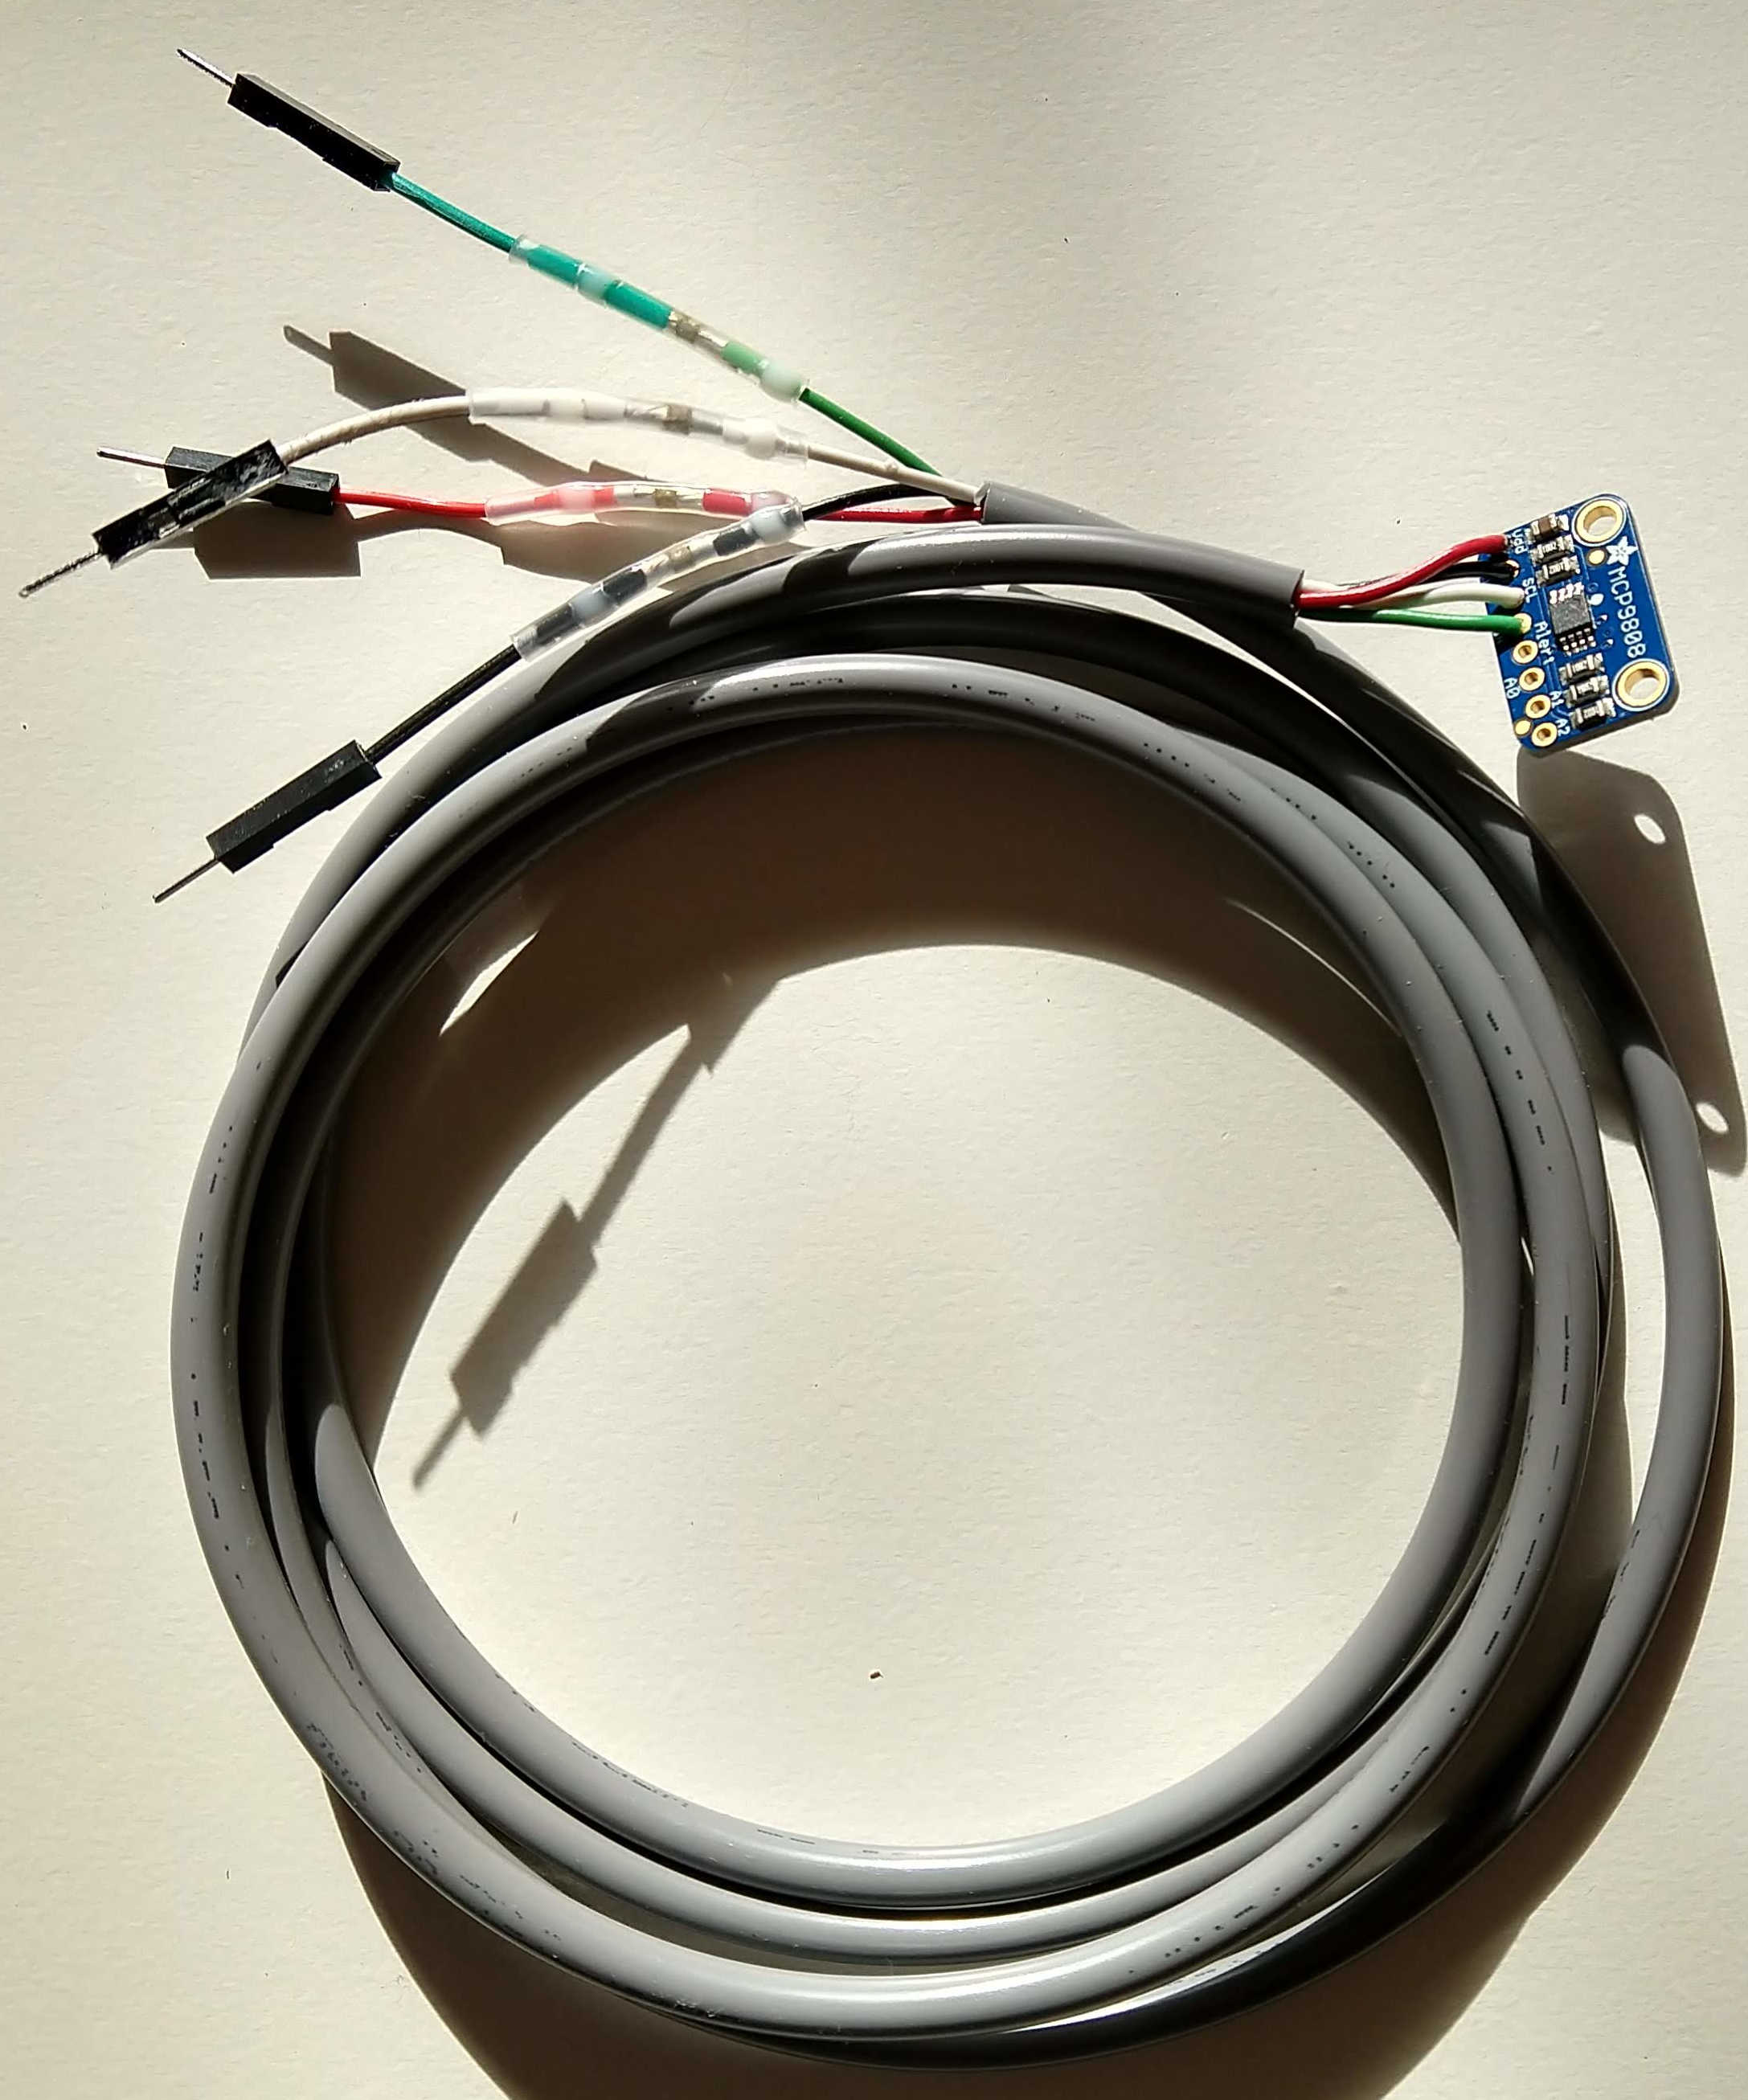
\includegraphics[width=\MFW]{Images/MCP9808_on_cable_cropped.jpg}}{https://github.com/publicsensors/IntroSensors/blob/digital/Images/MCP9808_on_cable_cropped.jpg}
		%\includegraphics[height=5cm]{Images/DS3231breadboard.jpg}
		\caption[MCP9808 on breadboard]{An \MCP9808 temperature sensor soldered onto a cable with 4 conductors (red $\leftrightarrow$ \texttt{Vdd}, black $\leftrightarrow$ \texttt{GND}, white $\leftrightarrow$ \texttt{SCL} and green $\leftrightarrow$ \texttt{SDA}).
		Male jumper ends are connected to the other end of the cable with \glspl{ssw_connector}.
		Note that, for clarity, the jumpers on the other end of the cable have colors consistent with the corresponding wires attached to the sensor.}
		\labfig{mcp9808_cable}
	\end{center}
\end{marginfigure}


\begin{marginfigure}
	\begin{center}
		\htmladdnormallink{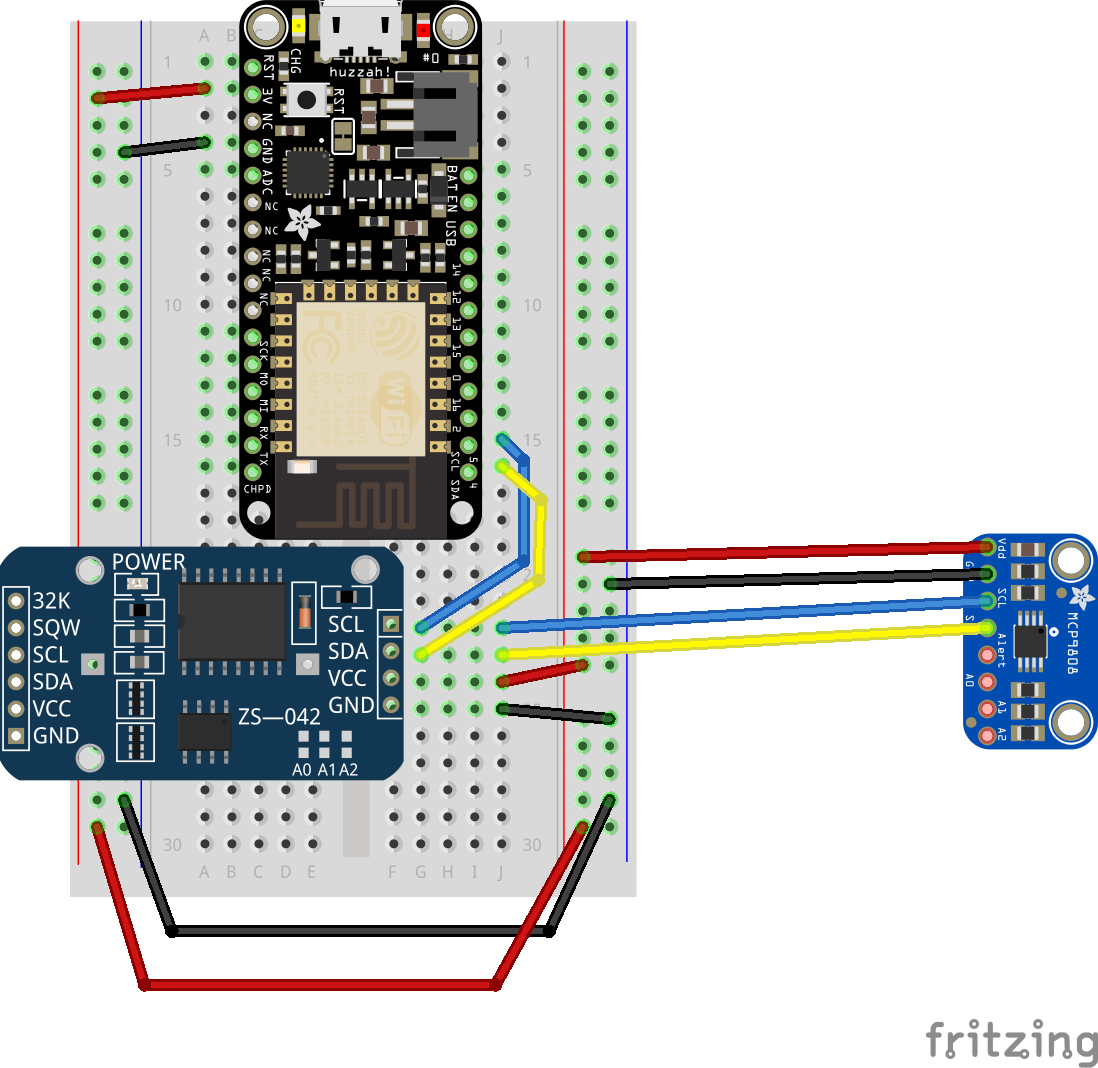
\includegraphics[width=\MFW]{Fritzing/feather_MCP9808_bb.png}}{https://github.com/publicsensors/IntroSensors/blob/digital/Fritzing/feather_MCP9808_bb.png}
		%\includegraphics[height=5cm]{Images/DS3231breadboard.jpg}
		\caption[MCP9808 on breadboard]{An example of layout and wire connections for the \MCP9808 temperature sensor and ESP8266 microcontroller. The circuit layout is similar to that used for the DS3231 external Real Time Clock. The DS3231 is left in the figure to emphasize that \i2c can support multiple devices simultaneously, but this exercise works equally well with or without the DS3231.}
		\labfig{mcp9808_breadboard}
	\end{center}
\end{marginfigure}


\begin{enumerate}
	\item \textbf{Connect wires to the GND, Vdd, SCL and SDA pins on the \MCP9808}.

	Like in the thermistor calibration in \refsec{cal_therm}, we will use ``water baths'' made of paper cups to expose the \MCP9808 sensors to known temperatures without getting them wet.
	This is most easily done if the sensor is connected to the microcontroller by extra long wires.

	\smallskip
	If your \MCP9808 has pins soldered to it, you can use two or more jumpers attached in series to give enough scope to move the sensor around.
	If your sensor does not have pins, you can solder some on, or alternatively solder long wires directly to the sensor (\reffig{mcp9808_cable}).

	You can then connect the other ends of the wires to the breadboard by soldering pins or male jumpers onto them; \reffig{mcp9808_cable} shows an example of this.
	The cable in this figure was made with \glspl{ssw_connector}, a fast and convenient way to join and protect two wire ends.

	Alternatively, you can attach wires directly to terminals (\eg, like \htmladdnormallink{these}{https://www.adafruit.com/product/2137?gclid=CjwKCAjwq9mLBhB2EiwAuYdMtZGP6ggrSAALQm8J7sbJ8Mwr6zWCWucqFVLvuSnaAGO22bPzFGNxmhoCVvEQAvD_BwE}), that then insert into breadboards.


	\item \textbf{Connect the GND and 3V pins on the ESP8266 to the GND and Vdd pins on the \MCP9808}.

	The circuit layout for the \MCP9808 is shown in \reffig{mcp9808_breadboard}.


	\item Connect the \texttt{SDA} (\#4) pin on the ESP8266 to the \texttt{SDA} pin on the \MCP9808, and the  \texttt{SCL} (\#5) pin on the ESP8266 to \texttt{SCL} on the \MCP9808.
	\item \textbf{Download the driver module provided on github by \texttt{@kfricke} called \htmladdnormallink{mcp9808.py}{https://raw.githubusercontent.com/kfricke/micropython-mcp9808/master/mcp9808.py} for the \MCP9808 temperature sensor.}

	Save it into a \texttt{Codes} directory on your computer.

	\item \textbf{Copy } \lstinline{mcp9808.py} \textbf{onto your microcontroller, using \thonny, \texttt{WebREPL} or \mpfshell (see the methods from \refch{connect} if you have questions).}
	\item %You are now ready to test your \DS3231 \rtc.
	\textbf{Set up the \i2c connection to your \MCP9808:}
\begin{lstlisting}[language=Python]
from machine import I2C, Pin
import mcp9808

i2c=I2C(scl=Pin(5),sda=Pin(4))
temp_mcp9808=mcp9808.MCP9808(i2c=i2c)
\end{lstlisting}
	\item \textbf{Set the resolution on your \MCP9808 to the highest possible}, with:
\begin{lstlisting}[language=Python]
temp_mcp9808.set_resolution(mcp9808.TEMP_RESOLUTION_MAX)
\end{lstlisting}

	\item \textbf{Query the temperature from your \MCP9808}:

	Here, there are two choices:
	If your microcontroller can do floating point math, use
\begin{lstlisting}[language=Python]
temp_mcp9808.get_temp()
\end{lstlisting}
The result of this command is the temperature in degrees Celsius, expressed as a floating point number.

\smallskip
If your microcontroller cannot do floating point math, use
\begin{lstlisting}[language=Python]
temp_mcp9808.get_temp_int()
\end{lstlisting}
The result of this command is two numbers.
The first is the temperature in whole degrees Celsius, expressed as an integer.
The second is the remaining fraction of a degrees Celsius, expressed as another integer.

\end{enumerate}
\loadMilestone{mlst:05a} % load milestone with tags id: mlst:04c


\subsection{\color{gray} Multiple sensors on a device: Temperature and pressure on an MS5803 \color{black}}

\subsection{\color{gray} Resolving \i2c address conflicts with a multiplexer \color{black}}
The requirement that each device on an \i2c bus has a unique address sometimes leads to address conflicts, in which two or more sensors have the same address.
Sometimes it is possible to create additional \i2c buses, dividing the duplicated address between them.
However, this is often not practical, especially when more than two devices share an address or when the number of \texttt{GPOI}s is limited.
Some \i2c devices have two or more addresses, which can be selected using jumpers between pins on thedevices.
Altering one sensor's address in this way is often a workable solution to address conflicts.
However, many i2c sensors have fixed addresses.
Furthermore, in an instrument designed to operate in the environment, sensors are often ``potted'' in epoxy or a sealant, or otherwise enclosed to protect them from water, salt, dust, \etc
These sensors typically are difficult or impossible to access to alter pin connections that shift \i2c addresses.

In these cases, an alternative strategy is provided by an \i2c \emph{multiplexer}.
An \i2c multiplexer is an \i2c device, which creates several (typically 8) \i2c ``sub-buses''.
The multiplexer allows i2c communications from only one sub-bus at a time -- which one is determined by a software command sent to the multiplexer by the microcontroller.
This means that two \i2c devices can be on different sub-buses, and because only one is operating at a given time there is no conflict even if they share the same address.

The details are best conveyed by an example:

The effect of light energy on many biological and physical processes is strongly affected by from which part of the spectrum it comes -- that is, it's \texttt{color}, taken to include wavelengths invisible to humans such as \gls{irLabel} and \gls{uvLabel}.
Under water, in forest canopies, at dawn or dusk or at high latitudes, and in many other situations it is potentially important to characterize light intensity as a function of color.
A \htmladdnormallink{TCS34725}{https://cdn-shop.adafruit.com/datasheets/TCS34725.pdf} color sensor, such as \htmladdnormallink{this one made by Adafruit}{https://www.adafruit.com/product/1334}, measures the \htmladdnormallink{RGB}{https://en.wikipedia.org/wiki/RGB_color_model} components of incident light.
However, to accurately characterize these primary colors, its light sensors are equipped with optical filters that exclude \gls{irLabel} wavelengths.
The \htmladdnormallink{TSL2591}{https://cdn-learn.adafruit.com/assets/assets/000/078/658/original/TSL2591_DS000338_6-00.pdf?1564168468} color sensor, such as \htmladdnormallink{also made by Adafruit}{https://www.adafruit.com/product/1980}, measure both full spectrum light intensity and the \gls{irLabel} component of that intensity.
So, simultaneous readings from both these sensors would characterize the blue, green, red and \gls{irLabel} component light intensities.

However, these sensors share the same \i2c address, so both cannot function simultaneously on the same \i2c bus.

\subsubsection{\howto Set up a TCA9548A \i2c multiplexer}

\begin{marginfigure}[-14cm]
	\begin{center}
		\htmladdnormallink{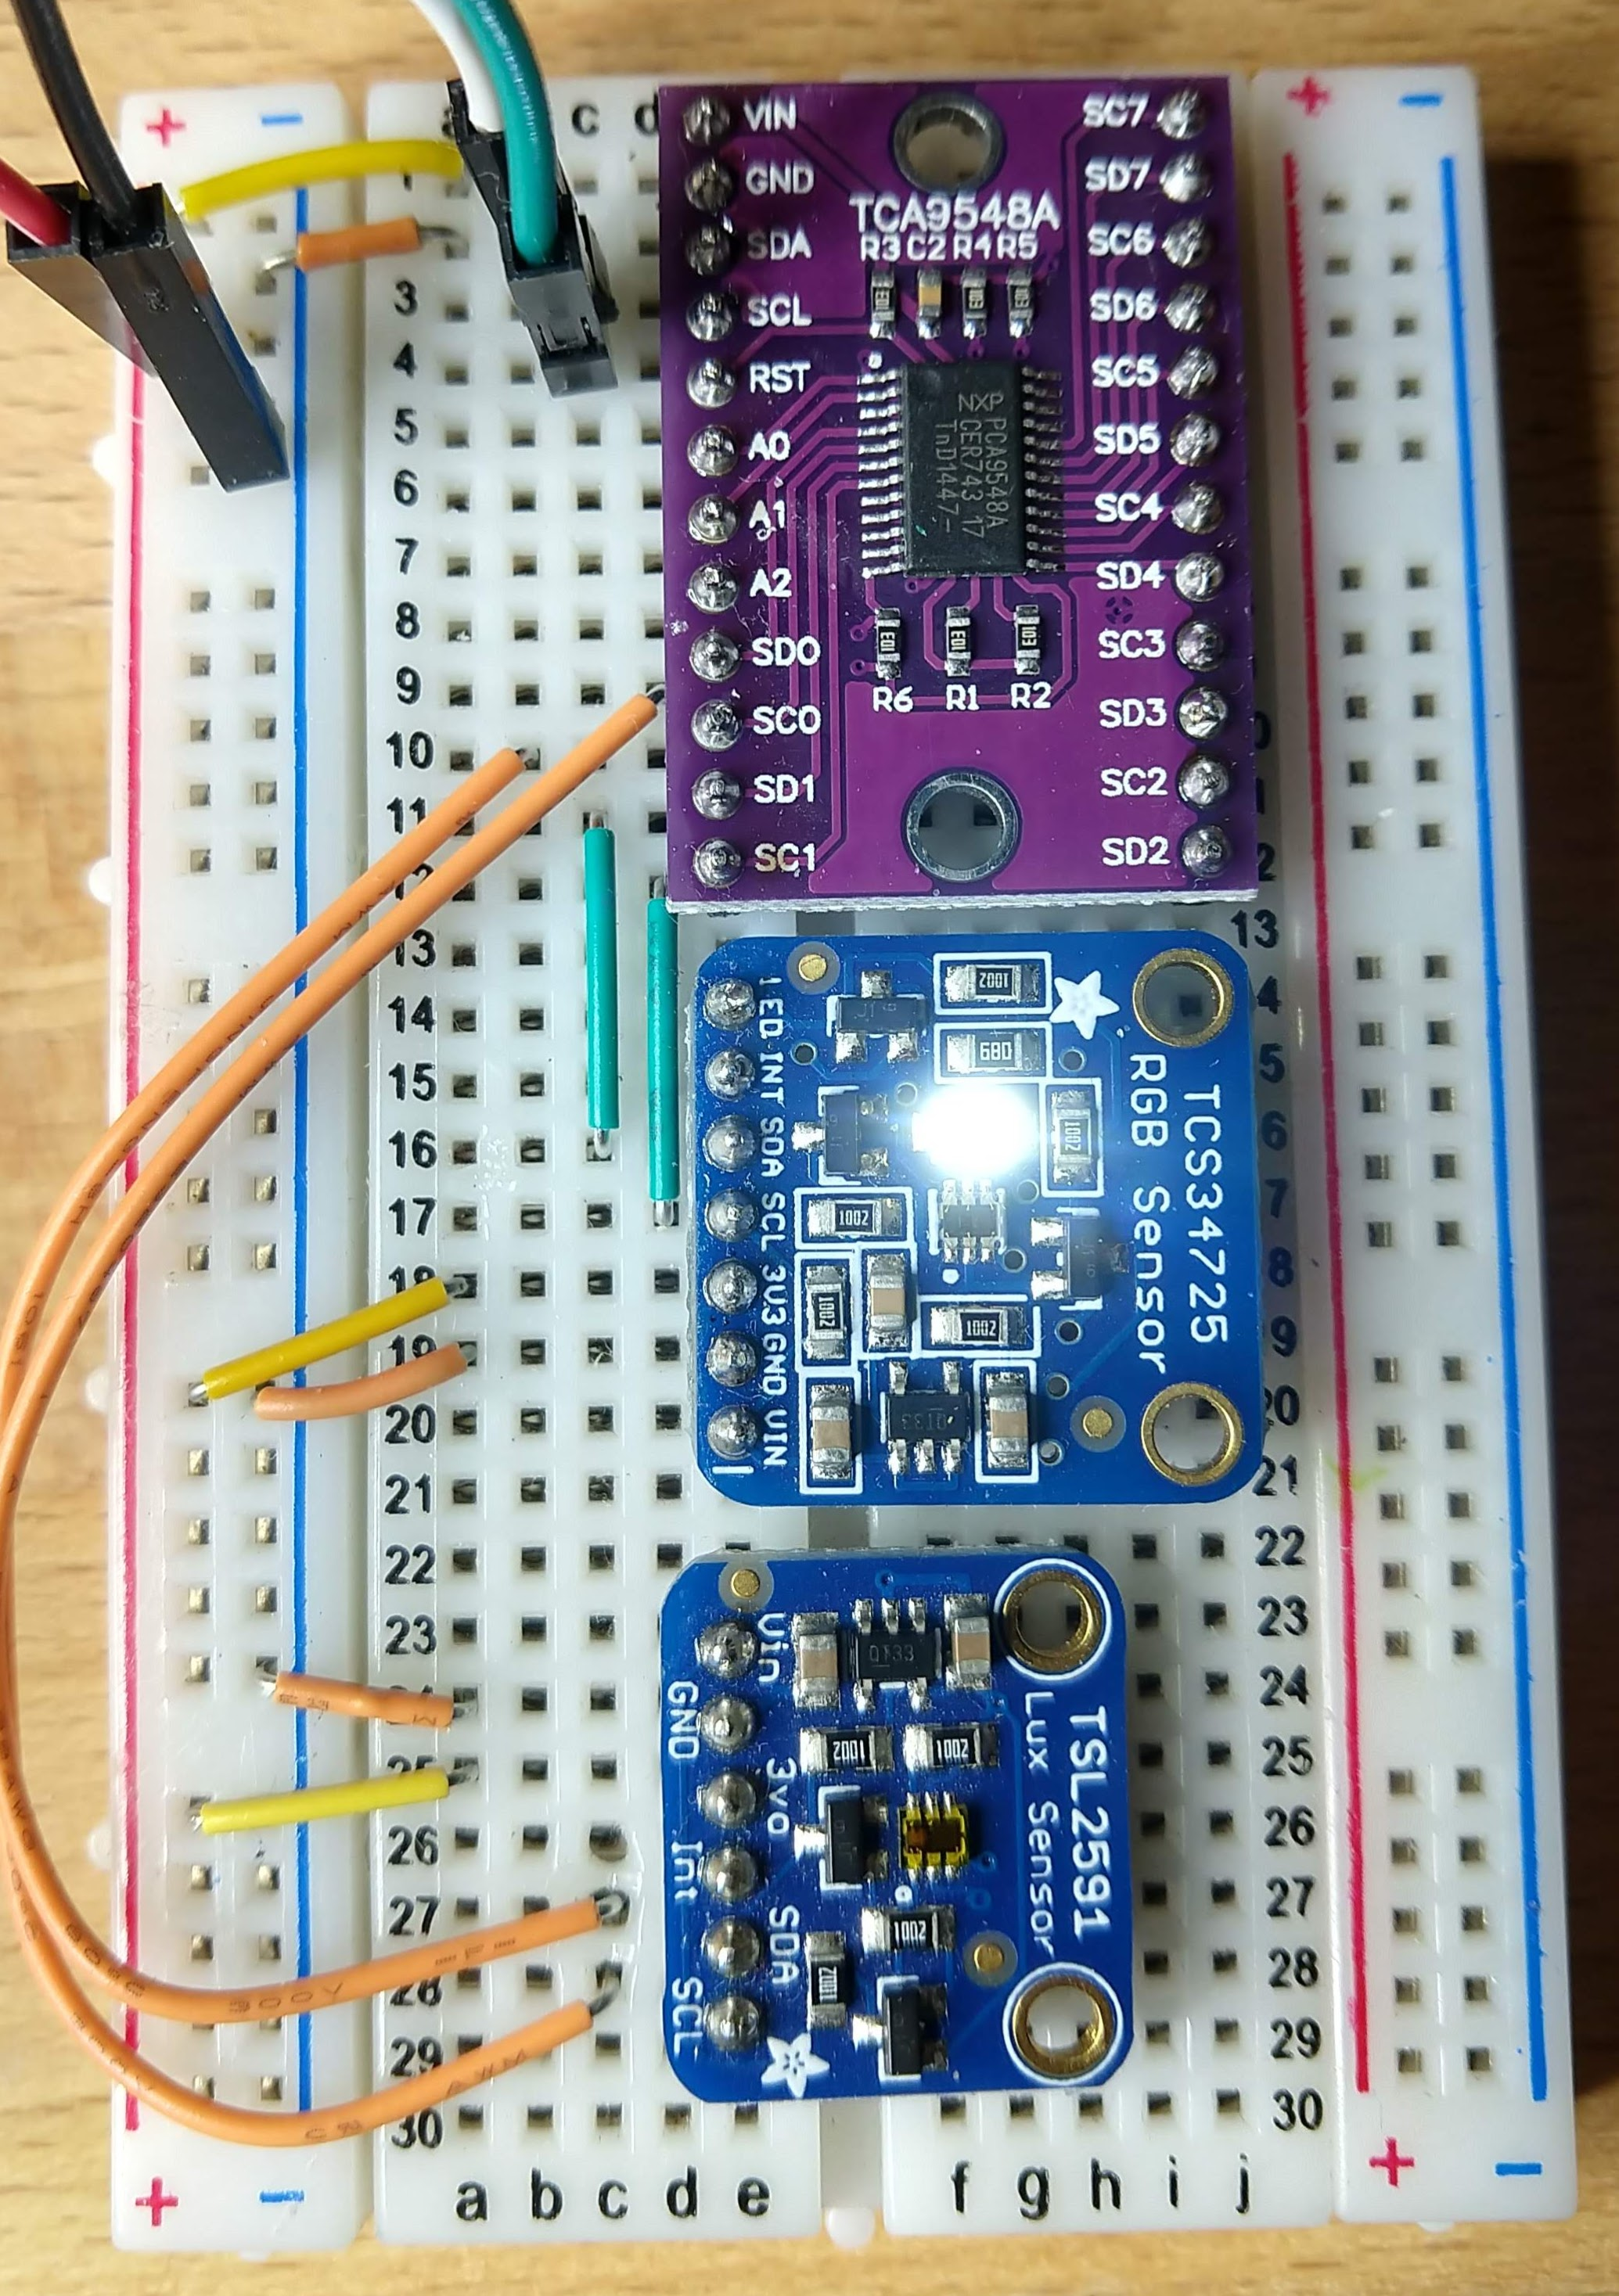
\includegraphics[width=\MFW]{Images/i2c_multiplexer_circuit.jpg}}{https://github.com/publicsensors/IntroSensors/blob/digital/Images/i2c_multiplexer_circuit.jpg}
		\caption[TCA9548A \i2c multiplexer circuit]{A TCA9548A \i2c multiplexer is used in this circuit to enable both a TCS34725 color sensor and a TSL2591 full spectrum/\gls{irLabel} sensor to operate on the same \i2c bus, even though they share the same \i2c address. The jumpers at the upper left lead to the microcontroller (red $\leftrightarrow$ \texttt{3V3}, black $\leftrightarrow$ \texttt{GND}, white $\leftrightarrow$ \texttt{SCL} and green $\leftrightarrow$ \texttt{SDA}. The white dot at the center is the built-in LED on the TCS34725, used to provide a standard illumination spectrum in some types of color measurements.}
		\labfig{i2c_mulitplx}
	\end{center}
\end{marginfigure}

A solution using a TCA9548A \i2c multiplexer is shown in \reffig{i2c_mulitplx}.
To use this circuit, we can use a modification of code posted on the \htmladdnormallink{MicroPython forum}{https://forum.micropython.org/viewtopic.php?t=6284} as a driver for the TCA9548A:
\lstinputlisting[language=Python,label=TCA9548Adriver,caption={\htmladdnormallink{\texttt{tca9548a.py}}{https://github.com/publicsensors/IntroSensors/blob/main/Codes/tca9548a.py}: A short driver for the TSC9548A \i2c multiplexer.}]{Codes/tca9548a.py}
% \lstinputlisting[language=Python,label=SetTimeDS3231,caption={\htmladdnormallink{\texttt{SetTimeDS3231.py}}{https://github.com/publicsensors/IntroSensors/blob/main/Codes/SetTimeDS3231.py}: A Micropython utility to set a \DS3231 \rtc to time from a Network Time Protocol (NTP) server.}]{Codes/SetTimeDS3231.py}

The TCS34725 color and TSL2591 full spectrum/\gls{irLabel} sensors as laid out in the circuit in \reffig{i2c_mulitplx} can then be querrrrried with the following code:
\lstinputlisting[language=Python,label=I2Cmultiplexer,caption={\htmladdnormallink{\texttt{multiplex\textunderscore i2c.py}}{https://github.com/publicsensors/IntroSensors/blob/main/Codes/multiplex_i2c.py}: An example use of  a TCA9548A \i2c multiplexer to communicate with color and full spectrum/\gls{irLabel} sensors that have an \i2c address conflict.}]{Codes/multiplex_i2c.py}

Note that this code imports the drivers for the TSC34725 color sensor, \htmladdnormallink{tsc34725.py}{https://github.com/adafruit/micropython-adafruit-tcs34725}, and for the TSL2591 full spectrum/\gls{irLabel} sensor, \htmladdnormallink{tsl2591.py}{https://github.com/jfischer/micropython-tsl2591}, have been copied onto the microcontroller.

The output of this demonstration code is:
\begin{lstlisting}[language=Python]
>>> import multiplex_i2c
light_sample =  628.646
color_sample =  (15, 10, 9, 34)
light_sample =  628.646
color_sample =  (15, 10, 9, 34)
light_sample =  628.646
color_sample =  (15, 10, 9, 34)
light_sample =  628.646
color_sample =  (15, 10, 9, 34)
light_sample =  628.646
color_sample =  (15, 10, 9, 34)
light_sample =  628.646
color_sample =  (15, 10, 9, 34)
light_sample =  64.464
color_sample =  (3, 1, 1, 5)
light_sample =  121.91
color_sample =  (4, 2, 2, 7)
light_sample =  121.91
color_sample =  (4, 2, 2, 7)
light_sample =  628.646
color_sample =  (15, 10, 9, 34)
>>>
\end{lstlisting}

\loadMilestone{mlst:05b} % load milestone with tags id: mlst:04c

\subsection{\color{gray} Using I2C over long cables with differential extenders \color{black}}


\section{\color{gray}1-wire sensors \color{black}}
\labsec{1wire_sensors}
\subsection{\color{gray} Background \color{black}}
1-wire is a proprietary protocol design that, as the name implies, uses only one wire in addition to \texttt{Vin} and \texttt{GND}.
1-wire is used in relatively few sensor types, but is worth knowing about because one of those is an inexpensive and versatile \htmladdnormallink{temperature sensor}{https://datasheets.maximintegrated.com/en/ds/DS18B20.pdf} that is among the most useful available for environmental monitoring.

\smallskip
1-wire supports many (up to hundreds) of devices on a single cable, each of which can be independently queried for sensor readings because it has a unique ROM address.
1-wire supports lower (but still generally sufficient) data rates than \i2c, which (when properly configured) can operate over much longer cables.

\subsection{\color{gray} Temperature measurements with DS18B20 digital sensors \color{black}}
\subsection{\color{gray} Accuracy and precision of DS18B20 temperature sensors \color{black}}
\subsubsection{\color{gray} Improve the accuracy and precision of DS18B20 temperature measurements with recalibration \color{black}}
\subsubsection{\color{gray} Monitoring temperature changes across time \color{black}}



\section{\color{gray}\uart sensors \color{black}}
\labsec{UART_sensors}
\subsection{\color{gray} Background \color{black}}
	\uart supports communication between only two devices, and these devices must share common settings for a number of parameters. %(bit speed, character length, parity, and stop bits).
Common applications in environmental sensing include \texttt{GPS} receivers and Air Quality Index sensors.

\uart uses two wires (in addition to \texttt{Vin} and \texttt{GND}), one for transmitting and one for receiving.
In some applications (\eg, some \texttt{GPS} configurations) only one of these functions is utilized (\eg, transmit on the \texttt{GPS} and receive on the microcontroller) in which case only one of these wires is necessary.
\subsection{\color{gray} Measuring position and velocity using the Global Positioning System (GPS) \color{black}}


\section{\spi sensors}
\labsec{spi_sensors}
\subsection{Background}
\spi is a ``4 wire'' protocol (in addition to \texttt{Vin} and \texttt{GND}).
However, three of these can be shared by multiple devices on the same \spi bus (the fourth must be unique to each device), so in some applications it is helpfully compact.
Technical details about \spi are at \htmladdnormallink{WikiPedia}{https://en.wikipedia.org/wiki/Serial\_Peripheral\_Interface\_Bus} and many other sources on the Internet.
One of the most useful explanations of the \spi protocol, in relation to \i2c and \uart, is provided by \htmladdnormallink{Sparkfun}{https://learn.sparkfun.com/tutorials/serial-peripheral-interface-spi/all}.

A single \spi bus can support multiple devices, each of which can transmit and receive data individually.
The focal device is specified by a ``chip select'' signal (over that 4th wire which is unique to each device).
This means there are no addressing conflicts, as can occur with \i2c.
Maximum data rates are higher for \spi than for \i2c or \uart devices.
Some digital sensors have both \spi and \i2c interfaces, so they can be used with either protocol.

As with \i2c, most microcontrollers have a built-in hardware \spi bus.
However, it is also often possible to ``bit-bang'' a software \spi bus, if the hardware \texttt{GPIO}s are not available.

%\sidenote[][*-12]{
	\begin{kaobox}[frametitle=Name that pin!]
		If there is a difficulty about the \spi interface, it is the variability in names for some of the \texttt{GPIO} connections.
		An \spi bus has one controlling device (almost always the  microcontroller), which sets the clock rate and determines which device is transmitting and receiving data at a given time.
		Originally, the connectors over which data are transmitted were called \texttt{MOSI} and \texttt{MISO}.
		That stood for ``Master Out, Slave In'' and ``Master In, Slave Out''.
		Because many users (the authors among them) \htmladdnormallink{found this nomenclature offensive}{https://www.oshwa.org/a-resolution-to-redefine-spi-signal-names}, a number of other names have come into use.

		In the \htmladdnormallink{Sparkfun}{https://learn.sparkfun.com/tutorials/serial-peripheral-interface-spi/all} tutorial, the pins are labeled \texttt{COPI} and \texttt{CIPO}, for ``Controller Out, Peripheral In'' and ``Controller In, Peripheral Out''.
		This more benignly preserves a property of the original labeling, that labels on all devices are consistent.

		Because it is rare for any device other than the microcontroller to act as the controller, the names in datasheets and labels on components have in many cases been shortened.
		For example, on the \esp8266 Feather, the \gpios connected to the hardware \spi bus are labeled \texttt{MO} (``Microcontroller Out'') and \texttt{MI} (``Microcontroller In'') without reference to the device.
		On many recent \spi devices, the corresponding labels are \texttt{DO} (``Device Out'') and \texttt{DI} (``Device In''), without reference to the controller.

		This can be slightly confusing, because labels are different on the microcontroller and peripheral devices.
	  However, you can keep it clear by keeping in mind that, like in \uart devices, data that go \underline{out} of one device go \underline{into} another.
	  As this implies, the \texttt{MO} \gpio is connected to the \texttt{DI} device pin, and the \texttt{MI} \gpio is connected to the \texttt{DO} device pin.
	\end{kaobox}
%}


\subsection{Connecting a microSD card through an \spi interface}
The addition of removable storage like a microSD card can hugely increase the capabilities of a microcontroller-based environmental sensor.
One reason for that is capacity: Onboard storage space on most microcontrollers amounts at most to 10s to 100s of megabytes (the \esp8266 is especially memory-constrained), while modern microSD cards with 10s to 100s of gigabytes are inexpensive and widely available.
Even voluminous data like very long time series can usually be recorded without much concern about space limitations on media of this size.

Another reason is accessibility: A microSD card can be programmed, inserted into an instrument, and extracted to retrieve data without ever needing to connect a cable to the microcontroller.
Those data can be read with almost any computer with a card reader or USB port.
A third reason is redundancy: Keeping duplicate copies of important codes and data on both a microcontroller's flash memory and a microSD card means that, if either fails, the information is not lost.

Microcontrollers that have a built-in microSD card reader, like the \texttt{ESP32CAM}, often have those readers hard-wired through internal connections to an \spi bus.
For those that don't, like the \esp8266, external microSD card readers utilizing the \spi interface are remarkably compact and inexpensive (we have been using \htmladdnormallink{these}{https://www.pjrc.com/store/sd_adaptor.html}, costing \$2, for many years).

\subsubsection{\howto Set up an external microSD card reader via \spi}

\begin{marginfigure}
	\begin{center}
		\htmladdnormallink{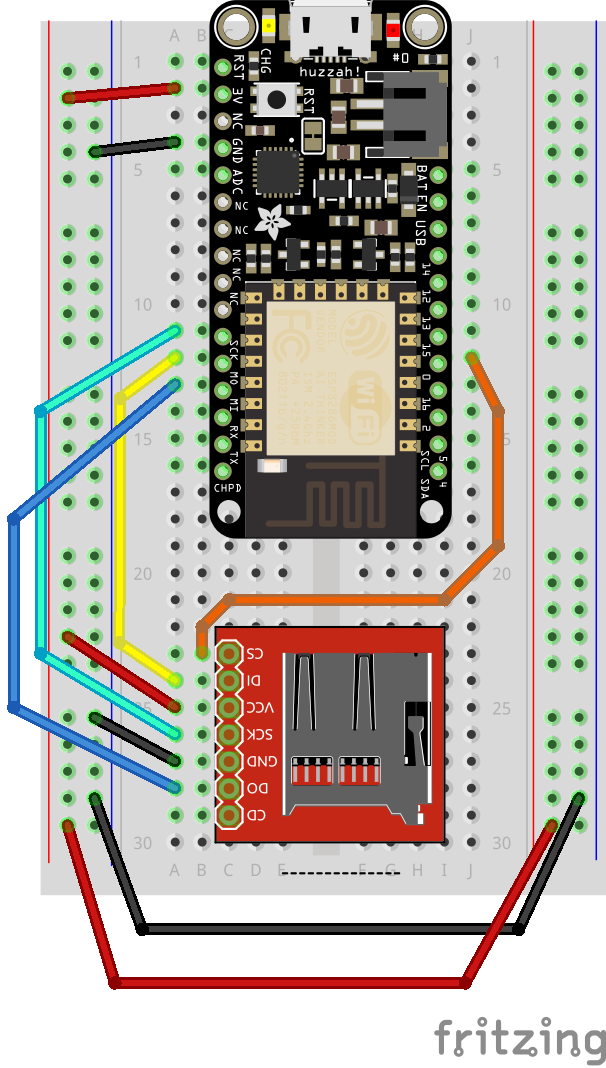
\includegraphics[width=\MFW]{Fritzing/feather_sdcard2_bb.png}}{https://github.com/publicsensors/IntroSensors/blob/digital/Fritzing/feather_sdcard2_bb.png}
		%\includegraphics[height=5cm]{Images/DS3231breadboard.jpg}
		\caption[microSD card on breadboard]{An example circuit with a microSD card reader connected to a microcontroller via the hardware \spi bus on an \esp8266 Feather.}
				\labfig{microSD}
	\end{center}
\end{marginfigure}

\begin{enumerate}
	\item \textbf{Connect pins or jumper wires to the GND, VCC, DO, DI, SCK and CS pins on the microSD card reader}.

	Note that there may be some variation in pin labeling.

	\item \textbf{Connect the GND and 3V pins on the ESP8266 to the GND and VCC pins on the microSD card reader}.

	The circuit layout for the \MCP9808 is shown in \reffig{microSD}.
	In this circuit, \texttt{GND} and \texttt{3V} are connected via the power rails, but any configuration that makes the apppropriate connections is OK.

	\item \textbf{Connect the \texttt{MI} pin on the ESP8266 to the \texttt{DO} pin on the microSD card reader. Similarly, connect \texttt{MO} to \texttt{DI} and \texttt{SCK} to \texttt{SCK}.}

	Note that, even though the \esp8266 Feather has \gpios labeled \texttt{MI}, \texttt{MO} and \texttt{SCK}, these are not actually separate pins.
	They are internally connected to \gpios on the other side of the microcontroller: the \texttt{MI} pin is really \gpio 12, \texttt{MO} is \gpio 13, and \texttt{SCK} is \gpio 14.

	\smallskip
	This means you can use \gpios 12, 13 and 14 to conect to the hrdware \spi bus, if they make your circuit layout more convenient.

	\smallskip
	On the other hand, \gpios 12, 13 and 14 are not available when using the hardware \spi bus, even if there is nothing directly connected to them.

	\item \textbf{Connect \gpio 15 on the ESP8266 to the \texttt{CS} pin on the microSD card reader.}

	This is the ``4th wire'', telling the reader when it is the device being addressed.
	It is fine to use another available \gpio, but make sure to modify the code below appropriately.

	\item \textbf{Download the driver for the SD card reader, \htmladdnormallink{sdcard.py}{https://raw.githubusercontent.com/publicsensors/IntroSensors/digital/Codes/sdcard.py}.}

	Save it into a \texttt{Codes} directory on your computer.

	\item \textbf{Copy } \lstinline{sdcard.py} \textbf{onto your microcontroller, using \thonny, \texttt{WebREPL} or \mpfshell (see the methods from \refch{connect} if you have questions).}

	This driver for \spi microSD card readers is part of the standard \Micropython library.
	However, it is omitted from most versions of firmware for the \esp8266, to save space.
	So usually you need to provide it on \esp8266 and some other smaller microcontrollers.

	\item \textbf{Format a FAT32 microSD card}

	It is possible to format a microSD ard using the reader itself, but we suggest you use your computer.
	For one thing, this makes it easy to see whether there are files you care about already on the card -- these will be irretrievably erased when the card is reformatted.
	It is also helpful in debugging, because it separates the formatting step from getting basic file writing and reading to work in a new circuit.

	\item \textbf{Copy a sample code onto the microSD card}

	This simple code will serve as an example and test of reading and executing code off the microSD card, rather than the microcontroller's built-in flash memory:
	\lstinputlisting[language=Python,label=sd_hello,caption={\htmladdnormallink{\texttt{sd\textunderscore hello.py}}{https://github.com/publicsensors/IntroSensors/blob/main/Codes/sd_hello.py}: An example to test reading and executing code from an SD card.}]{Codes/sd_hello.py}

	\item \textbf{Insert the FAT32 formatted microSD card into the reader}

	\item \textbf{Initialize the microSD card object}

	Type in and execute the following lines, one by one, into your microcontroller's \texttt{REPL}:
\begin{lstlisting}[language=Python]
import machine, sdcard, os, sys
sd = sdcard.SDCard(machine.SPI(1), machine.Pin(15))
os.mount(sd, '/sd')
os.listdir('/')
\end{lstlisting}
  With these commands, you performed three necessary steps.
  First, you imported modules that you will need to access the microSD card.
  Next, you created an sdcard object, named ``\texttt{sd}''.
  Then, you ``mounted'' the \texttt{sd} object into the filesystem as a subdirectory, under \texttt{/sd}.

  \smallskip
	The last command simply lists the files in the main directory on the microcontroller.
  The output should be a list of files, something like
\begin{lstlisting}[language=Python]
 ['sd', 'boot.py', 'main.py']
\end{lstlisting}
 The list should include whichever Python codes and other files or directories you have on your microcontroller.
 The main point now, however, is that you should see the \texttt{sd} entry appear.
 This shows that the microSD card is now visible to the filesystem.

	\item \textbf{Add the SD card to the filesystem path}

	The filesystem on your microcontroller has a list of locations in which it looks for codes to import.
	To see this list, execute the command
\begin{lstlisting}[language=Python]
sys.path
\end{lstlisting}
 The output will be something like
\begin{lstlisting}[language=Python]
['', '/lib', '/']
\end{lstlisting}
 This shows that the current locations in the filesystem in which the microcontroller looks for modules to import are the current working directory (''), the root of the filesystem ('/'), and a library subdirectory ()'/lib').
 Note that these do not include the microSD card, meaning codes on the card are not visible for import.

 \smallskip
 Now, execute:
 \begin{lstlisting}[language=Python]
sys.path.append("/sd")
sys.path
\end{lstlisting}
 The first of these adds "/sd" to the path list.
 The second prints out the augmented list, which should now include the microSD card:
\begin{lstlisting}[language=Python]
['', '/lib', '/', '/sd']
\end{lstlisting}
This shows that the microcontroller will now also look in the "/sd" subdirectory for modules to import.

	\item \textbf{Import the \texttt{sd\textunderscore hello.py} module from the microSD card}:
\begin{lstlisting}[language=Python]
import sd_hello
\end{lstlisting}
 The module should now load, giving the output:
\begin{lstlisting}[language=Python]
hello sdcard!
\end{lstlisting}

 If you got this output, you have successfully added a microSD card to your microcontoller's filesystem, and run code from it.
\end{enumerate}
\loadMilestone{mlst:05c} % load milestone with tags id: mlst:05c

% \subsection{\color{gray} SPI control of a TFT display panel \color{black}}


%
% \vspace{10cm}
%
%
% \section{Construction, calibration and use of a colorometric pH sensor}
% \labsec{pH_sensor}
% Placeholder for pH sensor section.
